\let\negmedspace\undefined
\let\negthickspace\undefined
\documentclass[journal]{IEEEtran}
\usepackage[a5paper, margin=10mm, onecolumn]{geometry}
\usepackage{lmodern} % Ensure lmodern is loaded for pdflatex
\usepackage{tfrupee} % Include tfrupee package

\setlength{\headheight}{1cm} % Set the height of the header box
\setlength{\headsep}{0mm}     % Set the distance between the header box and the top of the text

\usepackage{xcolor}

\usepackage{subfig}
\usepackage{cite}
\usepackage{amsmath,amssymb,amsfonts,amsthm}
\usepackage{algorithmic}
\usepackage{graphicx}
\usepackage{textcomp}
\usepackage{xcolor}
\usepackage{txfonts}
\usepackage{listings}
\usepackage{enumitem}
\usepackage{mathtools}
\usepackage{gensymb}
\usepackage{comment}
\usepackage[breaklinks=true]{hyperref}
\usepackage{tkz-euclide} 
\usepackage{listings}                                      
\def\inputGnumericTable{}                                 
\usepackage[latin1]{inputenc}                                
\usepackage{color}                                            
\usepackage{array}                                            
\usepackage{longtable}
\usepackage{multicol}
\usepackage{calc}                                             
\usepackage{multirow}                                         
\usepackage{hhline}                                           
\usepackage{ifthen}                                           
\usepackage{lscape}
\usepackage{float}


\title{\textbf{Clock Experiment using Arduino}}
\author{Ankit Jainar - EE24BTECH11004}
\date{\today}

\begin{document}

\maketitle


\tableofcontents
\newpage

\section{Introduction}
Explain the objective of the clock experiment and its significance in embedded systems. Provide a brief overview of Arduino and seven-segment displays.

\section{Components Used}

\begin{itemize}
 \item 6x Common-anode 7-segment displays
    \item 7447 BCD-to-7-segment decoder
    \item 6x 180$\Omega$ resistors 
    \item Jumper wires
    \item Bread Board
    \item Jumper wires for arduino and normal wires for seven segment displays
    \item Push Buttons
\end{itemize}

\section{Circuit setup}
The connections between the Arduino, 7-segment display, and other components as shown below
\subsection{7 Segment Display}
\begin{figure}[h]
    \centering
    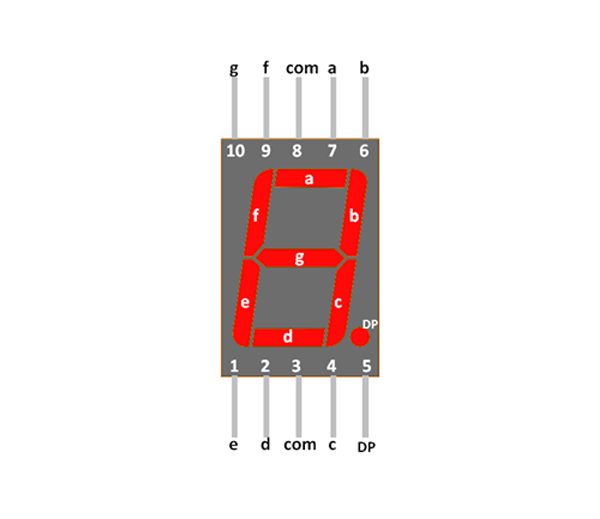
\includegraphics[width=0.5\textwidth]{figs/1.png} % Adjust width as needed
    \caption{7 Segment Display}
    
\end{figure}
\subsection{7447 IC}
\begin{figure}[h]
    \centering
    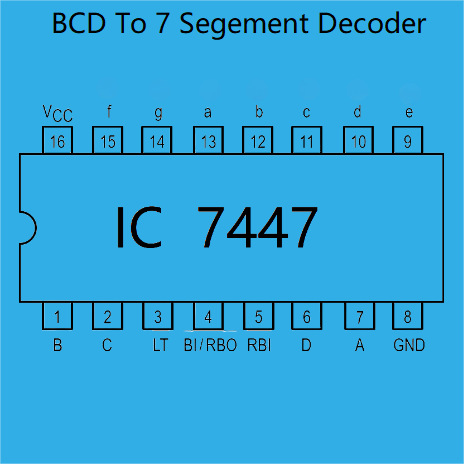
\includegraphics[width=0.5\textwidth]{figs/2.png} % Adjust width as needed
    \caption{7447 IC}
    
\end{figure}
\subsection{7447 Connections}
The table below shows the connections between the 7447 decoder and the Arduino Uno:

\begin{table}[H]
    \centering
    \caption{7447 to Arduino Pin Connections}
    \begin{tabular}{|c|c|}
        \hline
        \textbf{7447 Pin} & \textbf{Arduino Connection} \\
        \hline
        VCC (Pin 16) & +5V \\
        GND (Pin 8) & GND \\
        A (Pin 7) & D2 (BCD input LSB) \\
        B (Pin 1) & D3 \\
        C (Pin 2) & D4 \\
        D (Pin 6) & D5 (BCD input MSB) \\
        \hline
    \end{tabular}
\end{table}
\subsection{Segment Connections}
The 7447 outputs are connected to the corresponding segments of all six displays, as shown in the table below:

\begin{table}[H]
    \centering
    \caption{7447 to Display Segment Connections}
    \begin{tabular}{|c|c|}
        \hline
        \textbf{7447 Pin} & \textbf{Display Segment} \\
        \hline
        Pin 13 & Segment "a" \\
        Pin 12 & Segment "b" \\
        Pin 14 & Segment "c" \\
        Pin 15 & Segment "d" \\
        Pin 9  & Segment "e" \\
        Pin 10 & Segment "f" \\
        Pin 11 & Segment "g" \\
        \hline
    \end{tabular}
\end{table}

\subsection{Common Anode Connections}
Each display's common anode is connected to an Arduino analog pin through a 180$\Omega$ resistor to limit current flow.

\begin{table}[H]
    \centering
    \caption{Common Anode Connections}
    \begin{tabular}{|c|c|}
        \hline
        \textbf{Display} & \textbf{Arduino Analog Pin (via 180$\Omega$ resistor)} \\
        \hline
        Display 1 & A0 \\
        Display 2 & A1 \\
        Display 3 & A2 \\
        Display 4 & A3 \\
        Display 5 & A4 \\
        Display 6 & A5 \\
        \hline
    \end{tabular}
\end{table}

\section{Working Principle}
Describe how the Arduino generates the time signal, updates the display, and handles user input from the push buttons. Explain the role of the 7447 IC in decoding the BCD inputs.

\section{Code Implementation}
\section*{Key Features}
\begin{itemize}
    \item \textbf{Real-Time Interrupt-Driven Operation}: Timer1 is configured to trigger 1-second updates for consistent time management.
    \item \textbf{Interrupt Service Routine (ISR)}: Handles asynchronous updates to the Clock, Timer, and Stopwatch modes.
    \item \textbf{Multiplexed Display Control}: Efficient hardware management using binary-coded decimal (BCD) encoding and multiplexing.
    \item \textbf{Debounced Buttons}: Smooth user interaction for adjusting time settings and controlling modes.
    \item \textbf{Dynamic Mode Switching}: Seamlessly switches between Clock, Timer, and Stopwatch functionality using a mode variable.
\end{itemize}

\section*{ISR Overview}
The \textbf{Interrupt Service Routine (ISR)} is the backbone of the program, ensuring precise real-time operations. The Timer1 interrupt triggers every second, enabling reliable timekeeping and supporting the following functionalities:
\begin{itemize}
    \item \textbf{Clock Mode}: Implements a simple incrementing mechanism using \textbf{modulo arithmetic}, where seconds roll over after 60, minutes after 60, and hours after 24.
    \item \textbf{Timer Mode}: Uses a nested logic structure to decrement seconds, minutes, and hours. Special conditions ensure smooth transitions when seconds or minutes reach zero.
    \item \textbf{Stopwatch Mode}: Implements incrementing logic with rollover at 60 seconds and 60 minutes, similar to the Clock Mode. This is done to track elapsed time efficiently.
    \item \textbf{Debugging with PC7}: Toggles the \textbf{debugging LED} to ensure the ISR is running correctly and at expected intervals.
\end{itemize}

\section*{Hardware Overview}
\begin{itemize}
    \item \textbf{Registers}: \texttt{TCCR1B}, \texttt{OCR1A}, \texttt{PORTD}, \texttt{PORTC}, and \texttt{PINB}.
    \item \textbf{7-Segment Display}: Controlled using binary-coded decimal (BCD) encoding.
    \item \textbf{Buttons}: Connected to \texttt{PD6}, \texttt{PD7}, and \texttt{PB0/PB1} for mode switching and adjustments.
\end{itemize}

\section*{Code Snippets}
\subsection*{Timer Setup}
\begin{lstlisting}[language=C, frame=single, basicstyle=\ttfamily\small, keywordstyle=\color{blue}]
TCCR1B |= (1 << WGM12) | (1 << CS12) | (1 << CS10);
OCR1A = 15625; // 1-second interrupt
TIMSK1 |= (1 << OCIE1A);
sei(); // Enable global interrupts
\end{lstlisting}

\subsection*{Interrupt Service Routine (ISR)}
\begin{lstlisting}[language=C, frame=single, basicstyle=\ttfamily\small, keywordstyle=\color{blue}]
ISR(TIMER1_COMPA_vect) {
    // Toggle a debug LED to check ISR functionality
    PORTC ^= (1 << 7);

    // Clock Mode Logic
    if (mode == 0) { 
        seconds++;
        if (seconds == 60) { 
            seconds = 0; 
            minutes++; 
            if (minutes == 60) {
                minutes = 0;
                hours = (hours + 1) % 24; 
            }
        }
    }

    // Timer Countdown Logic
    if (mode == 1 && stopwatch_running) {
        if (timer_seconds > 0 || timer_minutes > 0 || timer_hours > 0) {
            if (timer_seconds == 0) {
                if (timer_minutes > 0) {
                    timer_minutes--;
                    timer_seconds = 59;
                } else if (timer_hours > 0) {
                    timer_hours--;
                    timer_minutes = 59;
                    timer_seconds = 59;
                }
            } else {
                timer_seconds--;
            }
        }
    }

    // Stopwatch Increment Logic
    if (mode == 2 && stopwatch_running) {
        stopwatch_seconds++;
        if (stopwatch_seconds == 60) {
            stopwatch_seconds = 0;
            stopwatch_minutes++;
            if (stopwatch_minutes == 60) {
                stopwatch_minutes = 0;
                stopwatch_hours = (stopwatch_hours + 1) % 24;
            }
        }
    }
}
\end{lstlisting}



\subsection*{Multiplexed Display Control}
\begin{lstlisting}[language=C, frame=single, basicstyle=\ttfamily\small, keywordstyle=\color{blue}]
void displayTime() {
    int digits[6];

    if (mode == 0) { // Clock Mode
        digits[0] = hours / 10;
        digits[1] = hours % 10;
        digits[2] = minutes / 10;
        digits[3] = minutes % 10;
        digits[4] = seconds / 10;
        digits[5] = seconds % 10;
    } else if (mode == 1) { // Timer Mode
        // Timer digits logic
    } else { // Stopwatch Mode
        // Stopwatch digits logic
    }

    // Multiplex 7-segment display
    for (int i = 0; i < 6; i++) {
        setBCD(digits[i]); // Send the BCD value
        COMMON_PORT = (1 << i); // Enable the corresponding digit
        _delay_us(500); // Short delay for smooth display
    }
}
\end{lstlisting}


Explain the key parts of the code like timer interrupts, BCD output logic, and display refresh.

\section{Results}

\subsection{Clock Mode}
In the Clock Mode, the system accurately maintains real-time hours, minutes, and seconds using the Timer1 interrupt. The display increments correctly at each second, with the hours resetting to zero after reaching 24. The implementation of modulo arithmetic ensures seamless rollover and precise time management.

\subsection{Timer Mode}
The Timer Mode was successfully tested for countdown scenarios. The nested logic structure managed the decrementing of seconds, minutes, and hours without any anomalies. Upon reaching zero, the timer stopped, demonstrating accurate time tracking. The use of edge cases, such as transitioning from 00:00:01 to 00:00:00, was handled effectively.

\subsection{Stopwatch Mode}
In Stopwatch Mode, the system recorded elapsed time reliably. Seconds and minutes were incremented accurately, with a correct rollover at 60. The stopwatch implementation, including the toggle for starting and stopping, was validated through multiple test scenarios. Overflow management ensured that the hours wrapped around at 24.

\subsection{Display Performance}
The multiplexed display control functioned smoothly without any noticeable flickering. The delay of 500 microseconds in the displayTime() function ensured a stable visual output. The binary-coded decimal (BCD) conversion using the 7447 IC provided clear and correct digit representation on the seven-segment display.

\subsection{Interrupt Service Routine (ISR) Validation}
The ISR was validated using a debug LED connected to PC7, which toggled at each Timer1 interrupt. The LED blinked precisely once per second, confirming accurate timing and proper interrupt handling. Additional tests confirmed no observable drift in time over extended operation.

\subsection{Button Response and Debouncing}
The button-based controls for mode switching and time adjustments responded effectively. The implemented debouncing logic prevented false triggers and ensured stable input recognition. Mode transitions occurred without lag, and time adjustments were instantaneous.

\subsection{Overall Evaluation}
The clock experiment demonstrated robust performance in all three modes. The use of efficient multiplexing, accurate Timer1 interrupts, and seamless ISR management contributed to the system's reliability. The design successfully met the objectives of providing real-time timekeeping, countdown timing, and stopwatch functionality with user-friendly control.


\section{Conclusion}
The implementation of the clock using Arduino, seven-segment displays, and the 7447 IC was a success. The experiment demonstrated the effective use of Timer1 interrupts for real-time operations, accurate management of time in multiple modes, and seamless switching between clock, timer, and stopwatch functionalities. The use of BCD encoding and multiplexing ensured efficient display management, while the debounce logic provided reliable user input. Overall, the project achieved its objectives and serves as a practical example of embedded systems design and real-time applications

\section{References}
\begin{enumerate}
    \item Arduino Documentation: \texttt{https://www.arduino.cc/}
    \item Datasheet of 7447 IC
    \item YouTube resources
    \item code credit Charan - EE24BTECH11052
\end{enumerate}

\end{document}


